% !TEX root = ../../Dissertation.tex

\begin{refsection}
	
\chapter{Experimental and Theoretical Methods} \label{methods}


\section{Experimental Methods}

Experimental data on gas phase clusters in this dissertation were obtained from two techniques which are anion photoelectron spectroscopy and infrared multiphoton dissociation spectroscopy. The first technique, anion photoelectron spectroscopy, provides energy needed to remove one electron (usually valence electrons) from gas phase anionic clusters, while the second one probes the infrared active vibration modes of atoms in clusters. The basic ideas behind these techniques are presented in the following subsections.   




\subsection{Anion photoelectron spectroscopy}

Photoelectron spectroscopy, historically known as Photoemission spectroscopy, is one of the most important methods used to investigate the electronic structure of molecules, clusters, surfaces, and solids.\cite{c1:reinert2005} The earliest experiment, which showed the effect of light on solids, was observed in 1887.\cite{c1:reinert2005} This is considered as the starting point of photoemission spectroscopy. Less than two decades later, in 1905, the concepts of photon and its energy were presented by Einstein. These theories set the ground for experiments in the early 1960s, that led to the modern photoelectron spectroscopy.\cite{c1:Spicer1964, c1:berglund1964, c1:Turner1962} Nowadays, photoelectron spectroscopy is categorized in two main types, X-ray photoelectron spectroscopy (\acrshort{xps}) and ultraviolet photoelectron spectroscopy (\acrshort{ups}). The division is made based on the different wavelengths used in these two methods and their application scope. \acrshort{ups} uses far-ultraviolet radiation with an energy large enough to remove valence electrons, while the higher energy X-ray employed on \acrshort{xps}, which is X-ray with higher energy, can ionize the core. %electrons. 



Since the spectroscopic data referred to in this thesis were measured by \acrshort{ups}, we will briefly introduce this technique. As mentioned above, the energy source of \acrshort{ups} can remove electrons from the valence states of the samples, and hence this method is used to determine the detachment energy of atomic and molecular systems. In a \acrshort{ups} spectrum, there are, normally, several peaks or bands corresponding to specific levels of detachment energies. Those bands are denoted by capital letters such as X, A, B, and C in order of increasing energy levels. Figure \ref{fig:c1:cr2o2spectrum} shows the photoelectron spectrum of \ch{Cr2O2-}, in which there are five bands noted as X to D and a very low-intensity band X'. Any single band allows for determination of the corresponding energy of ionization or electron detachment. 


\begin{figure}[htpb!]
	\centering
	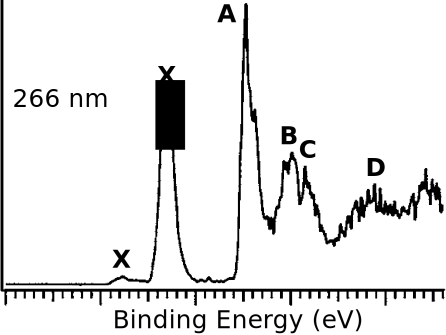
\includegraphics[width=0.5\linewidth]{Photoelectron-spectrum}
	\caption{The anion photoelectron spectrum of \ch{Cr2O2-} at 266 nm (reproduced with permission from ref \citenum{Zhai06}, Copyright 2006, AIP Publisher).}
	\label{fig:c1:cr2o2spectrum}
\end{figure}

The detachment energy (\acrshort{de}) withdrawn from photoelectron spectra, adiabatic detachment energy (\acrshort{ade}) and vertical detachment energy (\acrshort{vde}), is defined as:

\begin{equation}
		\acrshort{de} = E_{in} - E_{fi} 
\end{equation}

\noindent where $E_{in}$ and $E_{fi}$ are the energies of the initial and final states, respectively. From the theoretical aspect, to calculate \acrshort{ade} the geometric structure of the initial state and the final state are both optimized before calculating the energies. In case of \acrshort{vde}, energy of the final state is computed on the basis of the optimized geometry of the initial state. From the experimental perspective, DE can be calculated from the energy difference of laser source and kinetic energy of removed electrons. 

\begin{equation}
		\acrshort{de} = E_{photon} - E_{kinetic} = h\nu - \frac{1}{2}mv^2
\end{equation}

\noindent where E$_{photon}$ is the energy of laser photons defined as $h\nu$ and E$_{kinetic}$ is the kinetic energy of detachment electrons expanded as $\frac{1}{2}mv^2$. In some situations, the vibrational frequencies of the system in its final state can be extracted from the photoelectron spectra. 


The visible bands in photoelectron spectra correspond to transitions with a  non-zero transition dipole moment. Equation \ref{eq:probability} defines the transition dipole moment for a molecule or cluster absorbing a photon  

\begin{equation}
\mu=\Braket{\Psi^{\prime\prime}|\hat{\mu}|\Psi^{\prime}} 
\label{eq:probability}
\end{equation}

\noindent where $\hat{\mu}$ is the dipole operator including the electronic and nuclear dipole operators $\hat{\mu} = \hat{\mu}_{elec} + \hat{\mu}_{nuc}$, and $\Psi^{\prime}$ and $\Psi^{\prime\prime}$ are the total wave functions of the initial and final states, respectively. The total wave function of the initial and final states can be factorized into electronic, vibrational, and rotational parts. 

\begin{equation}
\Psi = \psi_{e}(\mathbf{r},\mathbf{R_e)}.\psi_{v}(\mathbf{R}).\psi_{r}(\mathbf{R})
\label{Eq:factorize}
\end{equation}

\noindent The vibrational $\psi_{v}(\mathbf{R})$ and rotational $\psi_{r}(\mathbf{R})$ parts of Equation \ref{Eq:factorize} depend on the coordinates of nuclei (\textbf{R}), while the electronic part $\psi_{e}(\mathbf{r},\mathbf{R_e)}$ depends on electron coordinates (\textbf{r}) and equilibrium coordinates of nuclei ($\mathbf{R_e}$) by application of the Born-Oppenheimer approximation.\cite{c1:Oppenheimer1927} By placing Equation \ref{Eq:factorize} into Equation \ref{eq:probability}, one obtains 

\begin{equation}
\begin{split}
\mu&=\Braket{\psi^{\prime\prime}_{e}(\mathbf{r},\mathbf{R_e)}.\psi^{\prime\prime}_{v}(\mathbf{R}).\psi^{\prime\prime}_{r}(\mathbf{R}) | {\hat{\mu}}_{elec} + {\hat{\mu}}_{nuc} | \psi^{\prime}_{e}(\mathbf{r},\mathbf{R_e)}.\psi^{\prime}_{v}(\mathbf{R}).\psi^{\prime}_{r}(\mathbf{R})}
\\&=\left\langle\psi^{\prime\prime}_{e}(\mathbf{r},\mathbf{R_e})|\hat{\mu}_{elec}|\psi^{\prime}_{e}(\mathbf{r},\mathbf{R_e})\right\rangle\left\langle{\psi^{\prime\prime}_{v}(\mathbf{R})|\psi^{\prime}_{v}(\mathbf{R})}\right\rangle\left\langle\psi^{\prime\prime}_{r}(\mathbf{R})|\psi^{\prime}_{r}(\mathbf{R})\right\rangle \\ 
&+ \left\langle\psi^{\prime\prime}_{e}(\mathbf{r},\mathbf{R_e})|\psi^{\prime}_{e}(\mathbf{r},\mathbf{R_e})\right\rangle\left\langle{\psi^{\prime\prime}_{v}(\mathbf{R})|\hat{\mu}_{nuc}|\psi^{\prime}_{v}(\mathbf{R})}\right\rangle\left\langle\psi^{\prime\prime}_{r}(\mathbf{R})|\hat{\mu}_{nuc}|\psi^{\prime}_{r}(\mathbf{R})\right\rangle
\end{split}
\end{equation}

\noindent Due to the orthogonality of the electronic wave functions on the initial and final states ($\left\langle\psi^{\prime\prime}_{e}(\mathbf{r},\mathbf{R_e})|\psi^{\prime}_{e}(\mathbf{r},\mathbf{R_e})\right\rangle = 0$) the transition dipole moment $\mu$ becomes

\begin{equation}
\mu =\left\langle\psi^{\prime\prime}_{e}(\mathbf{r},\mathbf{R_e})|\hat{\mu}_{elec}|\psi^{\prime}_{e}(\mathbf{r},\mathbf{R_e})\right\rangle\left\langle{\psi^{\prime\prime}_{v}(\mathbf{R})|\psi^{\prime}_{v}(\mathbf{R})}\right\rangle\left\langle\psi^{\prime\prime}_{r}(\mathbf{R})|\psi^{\prime}_{r}(\mathbf{R})\right\rangle
\label{eq:probability-2}
\end{equation}

\noindent Since the rotational part has a negligible effect on \acrshort{ups} spectra, it will not be considered. Therefore, the two remaining parts of Equation \ref{eq:probability-2} define electronic and vibrational selection rules for electronic transitions. The transition probability can be written as

\begin{equation}
\mu^2 =\left|\left\langle\psi^{\prime\prime}_{e}(\mathbf{r},\mathbf{R_e})|\hat{\mu}_{elec}|\psi^{\prime}_{e}(\mathbf{r},\mathbf{R_e})\right\rangle\right|^2\left|\left\langle{\psi^{\prime\prime}_{v}(\mathbf{R})|\psi^{\prime}_{v}(\mathbf{R})}\right\rangle\left\langle\psi^{\prime\prime}_{r}(\mathbf{R})|\psi^{\prime}_{r}(\mathbf{R})\right\rangle\right|^2
\label{eq:probability-3}
\end{equation}

\noindent From Equation \ref{eq:probability-3}, the electronic integral ($I_e$) and the Franck-Condon Factor (\acrshort{fcf}) can be defined as

\begin{equation}
I_e =\left|\left\langle\psi^{\prime\prime}_{e}(\mathbf{r},\mathbf{R_e})|\hat{\mu}_{elec}|\psi^{\prime}_{e}(\mathbf{r},\mathbf{R_e})\right\rangle\right|^2
\label{eq:electronic-part}
\end{equation}

\begin{equation}
FCF =\left|\left\langle{\psi^{\prime\prime}_{v}(\mathbf{R})|\psi^{\prime}_{v}(\mathbf{R})}\right\rangle\right|^2
\label{eq:CFC}
\end{equation}



The $\hat{\mu}_{elec}$ operator in Equation \ref{eq:electronic-part} is a one-electron operator for photoelectron transitions, and by applying the Slater-Condon rule,\cite{c1:21:Piela2014} we can prove that $I_e$ is non-zero when the photo-ionizations involve only one electron, and $I_e$ is not always the same for all electronic transitions. Since one electron is removed in the photoelectron process, the spin-\-mul\-tiplicity difference between the initial and final states is one ($\Delta S \pm 1/2$). For example, if an electron is removed from a quartet state, the final state will be a triplet or a quintet. In the one-electron detachment process, the arrangement of remaining electrons of the final state is the same as that of the initial state.




Since Equation \ref{eq:CFC} does not include the one-electron operator $\hat{\mu}$, the Franck-Condon Factor can be qualitatively predicted by employing symmetrical properties of the initial and final states' vibrational modes following the Franck–Condon principle. In general, the \acrshort{fcf} is zero if a non-totally symmetric integrand is obtained from Equation \ref{eq:CFC}. For polyatomic molecules, vibrational modes can be totally symmetric and non-totally symmetric. Concerning the former case, vibrational wave functions are always totally symmetric for all values of the vibrational quantum number $\upsilon$, and therefore the \acrshort{fcf}, theoretically, can be non-zero for any transitions between two vibrational wave functions ($\Delta\upsilon = 0, \pm1, \pm2, \ldots$). In contrast, for the case of non-totally symmetric vibrational modes, the vibrational wave function alternates from totally symmetric to non-totally symmetric as the vibrational number $\upsilon$ changes from even to odd. Hence, the \acrshort{fcf} will be non-zero for $\Delta\upsilon = 0, \pm2, \pm4, \ldots$. In both cases, it is possible to correlate the relative intensities of the peaks within a progression with the overlap (Equation \ref{eq:CFC}) between the vibrational wave functions of the involved states (Figure \ref{fig:c1:Franck-Condon-Principle}). Therefore, the transitions responsible for the most intense and sharp peaks of the spectra can be considered as vertical excitations where the motion of nuclei is negligible. The progression or band in photoelectron spectra will be very narrow, or even only one sharp peak if the normal coordinates of the initial and final states are not too much different. On the other hand, photoelectron bands will be broader when normal coordinate displacements between the initial and the final are large. In the cases of transitions involving large changes in normal coordinates, photoelectron bands will vanish from the spectra. In this dissertation, the MolFC program \cite{c2:molfc} was used to calculate \acrshort{fcf} defined in Equation \ref{eq:CFC}. 



%As long as the photodetachment process of one electron is very fast in comparison to motion of nuclei, the detachment of one electron is almost a vertical process

\begin{figure}[htpb!]
	\centering
	\includegraphics[width=0.6\linewidth]{Franck-Condon-Principle}
	\caption{Relative intensity of peaks within progressions. This is redrawn on the basis of Figure 7.2 from ref \citenum{c2:fcf}.}
	\label{fig:c1:Franck-Condon-Principle}
\end{figure}


\FloatBarrier


\subsection{Infrared Multiphoton Dissociation Spectroscopy} 

A molecule can be characterized by some primary properties such as molecular masses and chemical bonding (strength, angle, and length). All of these primary features can govern other related chemical and physical properties of a molecule. Vibration of molecules is one of related features governed by abovementioned primary properties. Under resonant absorption of photons, molecules will undergo vibrations and these vibrations are unique for a specific molecular structure. Such vibrations provide a unique fingerprint to identify geometric structures of specific molecules. The signals of these vibrations are recorded in vibrational spectra. Conventionally, vibrational spectra of molecules are measured by direct absorption of photons, and therefore this method is called direct \acrshort{ir} spectroscopy. Direct \acrshort{ir} spectroscopy has several shortcomings, and one of them is that this technique of \acrshort{ir} spectroscopy requires sufficient density of samples. As a result, this technique is usually used for liquid samples. For molecules and clusters in the gas phase, density of samples is much lower than that of samples in the liquid phase. Such low intensity of samples prevents direct \acrshort{ir} spectroscopy from application to gas phase clusters. Instead of that, \acrshort{ir} action spectroscopy was designed to overcome shortcomings of direct \acrshort{ir} spectroscopy.


Infrared multiphoton dissociation (\acrshort{irmpd}) spectroscopy is one of the popular techniques in the family of \acrshort{ir} action spectroscopy. This method is size selective and sensitive. This is due to \acrshort{irmpd} spectroscopy combines both mass spectrometry and \acrshort{ir} excitation. This is why \acrshort{irmpd} spectroscopy can be used for probing solid-state clusters at low density in the gas phase. Clusters are produced through the vaporization process of target solid samples under irradiation of a vaporization cluster source. After being cooled and expanded into vacuum, the distribution of formed clusters is analyzed by using a time-of-flight (TOF) mass spectrometer. The ion packet is, then, irradiated with the \acrshort{ir} laser pulse. When a cluster, so-called the mother cluster, absorbs photons with relevant levels of energy, this cluster or complex of clusters with messenger gases will be fragmented to form the product, namely the daughter cluster. Any change of masses (in the mother and daughter ones) in the cluster beam under \acrshort{ir} irradiation is traced to produce the depletion value which is then used to extract the absorption cross section, known as \acrshort{irmpd} signals. An experimental set-up coupled to “Free Electron Laser for Infrared eXperiments” (\acrshort{felix}) is visualized in Figure \ref{fig:IRPD-setup}. \acrshort{irmpd} spectra are obtained by scanning the wavelength of the intense \acrshort{ir} laser beam. An example of \acrshort{irmpd} spectra is given in Figure \ref{fig:IRPD-example}. More details of the \acrshort{irmpd} measurement and technique for specific kinds of clusters are provided in related chapters and ref \citenum{irpd}.       


\begin{figure}[htb!]
	\centering
	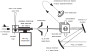
\includegraphics[width=0.9\linewidth]{IRPD-setup}
	\caption{Experimental set-up used for \acrshort{irmpd} measurements. This figure is taken from ref \citenum{irpd} with permission from Springer Publishing.}
	\label{fig:IRPD-setup} 
\end{figure} 


\begin{figure}[htb!]
	\centering
	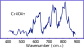
\includegraphics[scale=0.8]{IRPD-spectrum}
	\caption{\acrshort{irmpd} spectrum of the \ch{Cr4O4+} measured on the \ch{Cr4O4+}$\boldsymbol{\cdot}$Ne complex (reproduced with permission from ref \citenum{c2:cr4o4}, Copyright 2018, ACS Publisher).}
	\label{fig:IRPD-example} 
\end{figure} 










\section{Computational methods}

\subsection{Schr\"odinger Equation}
In 1926, with motivation from the de Broglie hypothesis about wave-like behaviors of matter, Erwin Schr\"odinger invented a partial differential equation derived from quantum mechanics describing the state of a physic system changing in time,\cite{c1:Schrodinger1926} the so-called Schr\"odinger equation. For stationary states, systems can be considered to be independent of time; and hence the Schr\"{o}dinger equation is written as the time-independent form:

\begin{equation}
\widehat{H}\mathrm{\Psi(\mathbf{r},\mathbf{R})} = E\mathrm{\Psi(\mathbf{r},\mathbf{R})}
\label{eq:Schrodinger}
\end{equation}

\noindent where $\widehat{H}$ is the Hamiltonian operator including electronic and nuclear parts of the physical system and E is an eigenvalue of Equation \ref{eq:Schrodinger} corresponding to the energy of the system.  $\widehat{H}$ is a differential operator acting on $\Psi(r,R)$, that can be formulated as Equation \ref{eq:Hamiltonian} in atomic units for a system of M nuclei and N electrons without magnetic or electric fields.

%In a system of M nuclei and N electrons without magnetic or electric fields, $\widehat{H}$ which is a differential operator acting on wave functions, can be formulated as Equation \ref{eq:Hamiltonian} in atomic units.

\begin{equation}
\widehat{H} = -\frac{1}{2}\sum_{i=1}^{N} \nabla_{i}^{2} -\frac{1}{2}\sum_{A=1}^{M} \frac{1}{M_A}\nabla_{A}^{2} - \sum_{i=1}^{N}\sum_{A=1}^{M}\frac{Z_A}{r_{iA}} + \sum_{i=1}^{N}\sum_{j>i}^{N} \frac{1}{r_{ij}} + \sum_{A=1}^{M}\sum_{B>A}^{M} \frac{Z_A Z_B}{R_{AB}}
\label{eq:Hamiltonian}
\end{equation}

\noindent Here, $ i $ and $ j $ run over the electrons, and A and B run over the nuclei. The first two terms in Equation \ref{eq:Hamiltonian} describe the kinetic energy of electrons and nuclei, and the Laplace operator $\nabla_{..}^{2}$ is a sum of differential operators with regard to Cartesian coordinates

\begin{equation}
\nabla_{..}^{2} = \frac{\partial^2}{\partial x_{..}^{2}} + \frac{\partial^2}{\partial y_{..}^{2}} + \frac{\partial^2}{\partial z_{..}^{2}}
\label{eq:laplacian}
\end{equation}

\noindent The three remaining terms in Equation \ref{eq:Hamiltonian} define the electron-nuclei attractive interaction, electron-electron potential and repulsive nuclei-nuclei interaction in the quantum system, respectively.

Since electrons are very light and move very fast in comparison to nuclei, the nuclei can be considered as fixed centers following the Born-Oppenheimer approximation.\cite{c1:Oppenheimer1927} As a result, the kinetic energy of the nuclei is zero and the repulsive potential due to nuclei-nuclei interaction is constant. Therefore, the only part that needs to be dealt with is the electronic one, so-called electronic Hamiltonian, instead of treating both nuclear and electronic parts in the Hamiltonian.
\begin{equation}
\widehat{H}_{elec} = -\frac{1}{2}\sum_{i=1}^{N} \nabla_{i}^{2} - 
\sum_{i=1}^{N}\sum_{A=1}^{M}\frac{Z_A}{r_{iA}} + \sum_{i=1}^{N}\sum_{j>i}^{N} 
\frac{1}{r_{ij}} = \widehat{T}_e + \widehat{V}_{Ne} + \widehat{V}_{ee}
\label{eq:HamiltonianElec}
\end{equation}

\noindent Thus, the Schr\"odinger equation becomes

\begin{equation}
\widehat{H}_{elec}\Psi_{elec} = E_{elec}\Psi_{elec}
\label{eq:SchrodingerElec}
\end{equation}

The solution of the Schr\"odinger equation in the Born-Oppenheimer approximation involves the electronic wave function $\Psi_{elec}$ and electronic energy $E_{elec}$. The total energy of the quantum system is therefore the sum of $E_{elec}$ and the nuclear repulsion term $E_{NN}$.

\begin{equation}
E_{tot} = E_{elec} + E_{NN}
\label{Eq:E_total}
\end{equation}

%\noindent If molecular dynamics are considered, the total energy of the system may have significant contributions from vibrational and rotational parts.

%in the form of a kinetic energy term $E_{Nk}$ involving the nuclei

%\begin{equation}
%E_{tot} = E_{elec} + E_{NN} + E_{Nk}.
%\label{Eq:E_total_Nk}
%\end{equation}

\subsection{Wave functions}

The electronic part (shortly noted as $\Psi(\mathbf{r})$) of the wave function in Equation \ref{eq:SchrodingerElec} is an abstract function. This abstract wave function has no universal form and itself has no physical meaning. However a physical attribute comes from the square modulus of the wave function $\left|\Psi(\vec{r}_1,\vec{r}_2,\cdots,\vec{r}_n)\right|^2$, which is the probability density of all electrons in positions $\vec{r}_1, \vec{r}_2, \-\cdots ,\vec{r}_n$.

To make the Schr\"odinger equation become practical, one must construct the electronic wave function in a specific form. Obviously, the wave function of a multi-electron system depends on all electrons of the system. Therefore, building up the wave function from all electrons of the system is meaningful. In an attempt to solve the Schr\"odinger equation, an approach for construction of the wave function was proposed by Hartree with the idea that the wave function could be factorized as a product of one-electron functions,\cite{c1:24:Szabo1996} which means that the motion of an electron is independent of that of other electrons.

\begin{equation}
	\label{c2:eq:Hatreeproduct}
\Psi(\vec{r}_1,\vec{r}_2,\cdots,\vec{r}_n) = \chi(\vec{r}_1)\chi(\vec{r}_2)\cdots\chi(\vec{r}_n)
\end{equation}

\noindent The wave function given in Equation \ref{c2:eq:Hatreeproduct} is known as the Hartree product. However, this factorized wave function does not satisfy the antisymmetry principle. To surmount this issue, Fock introduced a new way to derive the many-particle wave function $\Psi(\vec{r}_1,\vec{r}_2,\cdots,\vec{r}_n)$ using a Slater determinant. For a simple closed-shell electronic system, the wave function can be written as 

\begin{equation}
\Psi(\vec{r}_1,\vec{r}_2,\cdots,\vec{r}_n) = \Phi_{SD} =
\frac{1}{\sqrt{N!}}\left|\begin{matrix}
\chi_1(\vec{r}_1) & \chi_2(\vec{r}_1) & \cdots & \chi_N(\vec{r}_1) \\
\chi_1(\vec{r}_2) & \chi_2(\vec{r}_2) & \cdots & \chi_N(\vec{r}_2) \\
\vdots            & \vdots      	  & \ddots & \vdots            \\
\chi_1(\vec{r}_N) & \chi_2(\vec{r}_N) & \cdots & \chi_N(\vec{r}_N)
\end{matrix}\right|
\label{eq:SlaterWaveFucntion}
\end{equation}

\noindent or in a compact notation where only the diagonal elements are presented

\begin{equation}
\Phi_{SD} = \left|\chi_1(\vec{r}_1)\chi_2(\vec{r}_2)\cdots\chi_N(\vec{r}_N)\right|
\label{eq:SlaterWave_short}
\end{equation}

\noindent The one-electron functions $\chi_i(\vec{r}_i)$ are called \textit{spin orbitals} and are composed of two parts including a spatial orbital $\phi_{i}$ and a spin function $\sigma(s)$ ($\alpha(s)$ or $\beta(s)$), where $s$ is the spin coordinate taking two values of $\frac{1}{2}$ and -$\frac{1}{2}$.

\begin{equation}
\chi_{i} = \phi_{i}\sigma(s)
\label{eq:SpinOrbital}
\end{equation}

\noindent Describing the wave function of an open-shell electronic system is more demanding, as usually they require a linear combination of more than one Slater determinant. Other states of the electronic system, for example excited states, need more sophisticated approaches to reach accurate results.

\subsection{Hartree-Fock Method}

As mentioned above, the Hartree-Fock method considers the electrons to be independent of one another. To be clearer, electrons approximately move in an average electrostatic field arising from all other electrons.  By using  the Slater determinant for a closed-shell electronic system and applying the variational principle to the Schr\"odinger equation, the Hartree-Fock equations are obtained as

\begin{equation}
\widehat{f}\chi_i = \epsilon_i\chi_i, i = 1,2,\cdots, N
\label{eq:Hartree-Fock}
\end{equation}

\noindent where $\epsilon_i$ are the eigenvalues of the operator $\widehat{f}$. The $\epsilon_i$ are related to orbital energies and $\widehat{f}$ is the Fock operator defined as

\begin{equation}
\widehat{f}_i = -\frac{1}{2}\nabla_i^2 - \sum_{A}^{M}\frac{Z_A}{r_{iA}} + \widehat{V}_{HF}.
\label{eq:HF_operator}
\end{equation}



\noindent where $V_{HF}$ can be written in terms of the Coulomb and exchange operators as 

\begin{equation}
V_{HF} = \sum _{j=1}^N ( 2 \hat {J} _j -  \hat {K} _j )
\end{equation}

\noindent where $\hat {J} _j$ and $ \hat {K} _j$ are conveniently defined by application to a one-electron wave function 

\begin{equation}
\hat {J}_j (1) \chi _i (1) = \left [ \int \chi ^*_i (2) \dfrac {1}{r_{12}} \chi _i (2) d \tau _2 \right ] \chi _i (1)
\end{equation}


\begin{equation}
\hat {K}_j (1) \chi _i (1) = \left [ \int \chi ^*_j (2) \dfrac {1}{r_{12}} \chi _i (2) d \tau _2 \right ] \chi _j (1)
\end{equation}

The Hartree-Fock equations \ref{eq:Hartree-Fock} are solved iteratively. First, a set of guessed functions
($\chi_1, \chi_2, \cdots, \chi_n$) is used to calculate the set of effective potentials $V_{HF}$. The Hartree-Fock equations are solved to produce a set of improved functions $\chi_i$. These new functions serve to update the effective potentials, which in turn are used to calculate a new improved set of functions $\chi_i$ by solving the Hartree-Fock equations again. The cycles of calculations continued until the changes on functions $\chi_i$ are negligible. This is the so-called self-consistent field (\acrshort{scf}) method.

%owing to the fact that $V_{HF}(i)$ is only determined when all of the one-electron functions $\chi_i$ are known, however these one-electron functions $\chi_i$ are what need to be attained after solving Hartree–Fock equations. The technique used to solve Hartree–Fock equations is called \textit{self-consistent field} (\acrshort{scf}).

%There had been no systematic procedures to solve the Hartree–Fock equations. The only one solution would be to use numerical methods to obtain the results. To overcome this problem, Roothaan has proposed a new approach, which is the introduction of a finite basis set including atomic orbitals (\acrshort{ao}s) to expand the molecular orbitals. 

\subsection{ Restricted, Restricted Open-shell and Unrestricted wave functions}

As mentioned above, electrons have two options of spin functions $\alpha(s)$ or  $\beta(s)$. For closed-shell systems, each pair of electrons is treated with the same spatial orbital. This is called the \textit{restricted Hartree-Fock} method (\acrshort{rhf}). Most organic compounds and small molecules, for instance water or carbon dioxide, are closed-shell systems. Open-shell electronic states (radicals for example) can be described with an orbital set in which both doubly (by forcing electrons of opposite spin functions in the same spatial orbital) and singly occupied orbitals are used. This is the so-called \textit{restricted open-shell Hartree-Fock} method (\acrshort{rohf}). Finally, the unrestricted Hartree-Fock (\acrshort{uhf}) formalism describes each electron with its own spin and spatial function. These differences are illustrated in Figure \ref{fig:RHF_UHF}.

\begin{figure}[htb!]
	\centering
	\includegraphics[width=0.6\linewidth]{RHF-ROFH-UHF}
	\caption{Schematic representation of the electronic structure obtained with \acrshort{rhf} for a singlet state and \acrshort{rohf} and \acrshort{uhf} for a doublet state}
	\label{fig:RHF_UHF}
\end{figure}

\subsection{Basis Sets}

In order to solve the Schr\"odinger equation by the Hartree-Fock method with Root\-han's procedure,\cite{c1:22:Lewars2011} a set of basis atomic functions must be employed. Ideally, this set of basis functions should be infinite to obtain the lowest energy of the system for the corresponding wave function. Since it is not possible to work with an infinite set of basis functions, we work with finite basis sets.

Slater introduced in 1930 the so-called Slater type orbitals (STO),\cite{c1:slater1930} which are defined as Equation \ref{eq:Slater_type} in atom-centered polar coordinates

\begin{equation}
S_{\zeta,n,m,l}(r,\theta,\phi) = NY_{l,m}(\theta,\phi)r^{n-1}e^{-\zeta r}
\label{eq:Slater_type}
\end{equation}

\noindent in which N is a normalization constant and $Y_{l,m}$ are spherical harmonic functions that depend on the angular momentum and magnetic quantum numbers \textit{l} and \textit{m}. $Y_{l,m}$ functions are quite analogous to angular parts of the hydrogen atom's wave functions gathered from the solution of Schr\"odinger equation for the hydrogen atom.

Because Slater type atomic orbitals are similar to wave functions of the hydrogen atom, they are a very advantageous basis type to construct molecular orbitals. The \acrshort{sto}s have correct exponential change when r (the distance of the electron from the atomic nucleus) increases in comparison to the exact hydrogenic orbitals, and the 1s orbital has a cusp at the nucleus. However, \acrshort{sto}s are just suitable for single atoms or relatively small molecules because two-electron integrals with three and four different functions and three- and four-center cannot be performed analytically but numerically, which negatively affects its evaluation.

%Moreover, \acrshort{sto}s have no radial nodes, which is a shortcoming with regard of hydrogen-like orbitals.

In 1960, Boys \cite{c1:boys1950} introduced Gaussian functions in the so-called  Gaussian type orbitals (\acrshort{gto}s) for the first time, which can be written in polar coordinates as

\begin{equation}
G_{\zeta,n,m,l}(r,\theta,\phi) = NY_{l,m}(\theta,\phi)r^{2n-2-l}e^{-\zeta r^2}.
\label{eq:Gaussian_type}
\end{equation}

\noindent Basis functions $G_s$ can be primitive Gaussian functions or linear combination of primitive Gaussian functions to mimic \acrshort{sto}s, namely \textit{contracted} Gaussian functions.  

\begin{equation}
\varphi = \sum_{1}^{u} c_u G_u
\label{eq:contracted_Gaussian}
\end{equation}

\noindent where $c_u$ are contraction coefficients. The set of primitive or contracted functions forms a Gaussian basis set. Combinations of Gaussian primitives are able to approximate correct nodal properties of atomic orbitals and to describe the orbitals for atoms and molecules. However, contracted Gaussian functions have a zero slope at the nucleus, which is, consequently, a drawback of \acrshort{gto}s in representing the proper behaviour near the nucleus vis-\`a-vis \acrshort{sto}s.


Nowadays, an abundance of basis sets composed of \acrshort{gto}s are widely used in modern quantum packages. Each type of basis sets was designed for a specific element or computational method. Typical basis sets widely used are those of Pople (3-21G, 6-31G, 6-311G,...), Ahlrichs (def2-SVP, def2-TZVP, and def2-QZVP), Dunning (cc-PV$n$Z), and atomic natural orbitals (\acrshort{ano}) basis sets.


\subsection{Post Hartree-Fock Methods}

\subsubsection{Correlation Energy}

%The Hartree-Fock method has its own limit that it does not pay much attention to electron correlation, which leads to the inaccurate values of system energies. It is only about 1\% of system energies in electron correlation, nevertheless this amount of energies is crucial for explaining or estimating properties of quantum systems. The electron correlation energy ($ E_{corr} $) can be defined as the difference between the exact energy ($ E_{exact} $) and the energy calculated by the HF methods ($ E_{HF} $).

Since the Hartree-Fock method uses one Slater determinant, it lacks electron correlation, which is an effect that stems from electron-electron interaction. It is only about 1\% of the system total energy, but this amount is crucial for explaining or estimating properties of correlated quantum systems. The electron correlation energy ($ E_{corr} $) can be defined as the difference between the exact energy ($ E_{exact} $) and the energy calculated by the HF methods ($ E_{HF} $).

\begin{equation}
E_{corr} = E_{exact} - E_{HF}
\label{eq:Ecorrelation}
\end{equation}


Correlation energy $E_{corr}$ can be abstractly divided into two types, namely static and dynamic correlation. Static energy is known as the difference in energy between wave functions represented by a single Slater determinant (\acrshort{sd}) and a linear combination of \acrshort{sd}s. In many situations, a single SD cannot be used to represent the wave function of a system such as bond dissociation, excited states, and transition-metal compounds. Dynamic correlation energy is caused by instantaneous interaction among electrons. Recovering the $E_{corr}$ contribution is a difficult task that led to the development of sophisticated wave function based methods, or the so-called post Hartree-Fock methods.


\subsubsection{Configuration Interaction (\acrshort{ci})}

%Opposite with the Hartree-Fock method using a single determinant of "ground state" for the wave function in the Schr\"odinger equation, \acrshort{ci} in principle employs a linear combinations of all possible n-electron wave function configurations (Fig. \ref{fig:CI.configurations}) generated from the Hartree-Fock wave function.\cite{c1:sherrill1999} 

The \acrshort{ci} method \cite{c1:sherrill1999} expands the Hartree-Fock wave function, which uses a single Slater determinant, with an arbitrary number of determinants that form a linear combination of n-electron wave function configurations.

\begin{equation}
\Psi_{CI} = a_0\Phi_{HF} + \sum a_S\Phi_S + \sum a_D\Phi_D + \sum a_T\Phi_T  + \cdots = \sum a_i\Phi_i \label{eq:CI.wave function}
\end{equation}



\noindent The Hartree-Fock wave function is expanded with Slater determinants for electronic configurations arising from excitations of one, two or more electron(s) from  occupied orbital(s) to unoccupied one(s). These excited electronic configurations are often referred to as \textit{Singles} (S), \textit{Doubles} (D), \textit{Triples} (T), \textit{Quadruples} (Q), etc. and visualized in Figure \ref{fig:CI.configurations}.


\begin{figure}[htb!]
	\centering
	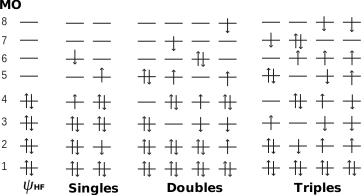
\includegraphics[width=0.7\textwidth]{CI-configurations}
	\caption{Possible configurations of first three excited states generated from a Hartree-Fock single configuration.}
	\label{fig:CI.configurations}
\end{figure}



Replacing \acrshort{ci} wave functions described by Equation \ref{eq:CI.wave function} into Equation \ref{eq:SchrodingerElec} and solving the resulting equation will recover some amount of $E_{corr}$. Nonetheless, the number of excited configurations becomes very high very fast, and it is infinite with a complete set of basis functions. Therefore, its solution becomes practically impossible when the linear combination Equation \ref{eq:CI.wave function} involves numerous excited determinants. Hence, in practice \acrshort{ci} methods are implemented at limited amount of excitations. For instance, a common approach is the so-called CISD method that only includes single and double excitations.

\begin{equation}
\Psi_{CI} = a_{0}\Phi_{HF} + a_S\Phi_{S} + a_D\Phi_{D}
\label{eq:CISD}
\end{equation}

\noindent Other levels of accuracy can be considered and added to Equation \ref{eq:CISD} to meet the demand if it is necessary.

\subsubsection{Perturbation Theory} \label{section:Perturbation}

In perturbation theory, a reference Hamiltonian $\widehat{H}^0$ is improved by applying a perturbation operator $\lambda\widehat{H}^\prime$ as in Equation \ref{eq:pert.Operator}.

%the difference $\lambda\widehat{H}^\prime$ between the true Hamiltonian $\widehat{H}$ of a system and the simpler model system's Hamiltonian $\widehat{H}^0$ is described in Equation \ref{eq:pert.Operator}.

\begin{equation}
\widehat{H} = \widehat{H}^0+ \lambda\widehat{H}^\prime
\label{eq:pert.Operator}
\end{equation}

\noindent where $\lambda$  varies from 0 to 1. If eigenvectors and eigenvalues of the reference operator $\widehat{H}^0$ are known and the contribution of $\widehat{H}^\prime$ is small in comparison to $\widehat{H}^0$, we can find the eigenvectors of the full operator as an expansion of the eigenvectors of $\widehat{H}^0$ and the corrected eigenvalues of the system. To be more specific, the first-order and second-order corrections to the energy are given by Equation \ref{eq:first-oder} and \ref{eq:second-oder}.

\begin{equation}
E^{(1)}_n = \left\langle\Psi^{(0)}_n\left|H^\prime\right|\Psi^{(0)}_n\right\rangle
\label{eq:first-oder}
\end{equation}


\begin{equation}
E^{(2)}_n = \sum_{m\neq n}\frac{\left|\left\langle\Psi^{(0)}_m\left\lvert H^\prime \right\rvert\Psi^{(0)}_n\right\rangle\right|^2}{E^{(0)}_n - E^{(0)}_m}
\label{eq:second-oder}
\end{equation}

\noindent M\o{}ller and Plesset applied perturbation theory to quantum systems by adding the perturbation operator to the Hartree-Fock Hamiltonian.\cite{c1:moller1934}  As a result, this will generate n-order corrections to the HF wave function and energy. The levels of M\o{}ller–Plesset (MP) perturbation theory are denoted as MPn (n = 0, 1, 2, $\cdots$). MP0 corresponds to the sum of all the Hartree–Fock one-electron energies, and MP1 is the HF level of energy (MP0 plus coulomb and exchange integral energy). We can write $E_{MP1} = E^{HF}_{total} = E_{MP0} + E^{(1)}$. MP2 is the first corrected level beyond the Hartree-Fock method:

\begin{equation}
E_{MP2} = E^{HF}_{total} + E^{(2)}
\label{eq:MP2}
\end{equation}



%The roles of n-order corrections (n $\geq$2) are states-like configurations discussed in Section \ref{section:Perturbation}, which is the correction of electron-electron correlation. 

\subsubsection{Coupled-Cluster Theory}
Coupled-cluster theory was developed in 1966 \cite{c1:vcivzek1966} and this is, notably, one of the most accurate methods for electron correlation energies of quantum systems. \acrshort{cc} theory describes the wave function as

\begin{equation}
\Psi = e^{\widehat{T}}\Psi_{HF}
\label{eq:CC_wave function}
\end{equation}

\noindent where $e^{\widehat{T}}$ is the exponential cluster operator defined as 

\begin{equation}
e^{\widehat{T}} = 1 + \widehat{T} + \frac{\widehat{T}^2}{2!} + \frac{\widehat{T}^3}{3!} + \ldots + \frac{\widehat{T}^k}{k!} \ (k = \infty)
\label{eq:E.Cluster_Taylor}
\end{equation}

\noindent and $\widehat{T}$ is the summation of operators $\widehat{T}_1, \widehat{T}_2,\ldots, \widehat{T}_N$

\begin{equation}
\widehat{T} = \widehat{T}_1 + \widehat{T}_2 + \ldots + \widehat{T}_N
\label{T_operator}
\end{equation}

\noindent Each $\widehat{T}_i$ acts on the \acrshort{hf} wave function to create all possible i-electron excited states from the ground-state wave function, for example


\begin{equation}
\widehat{T}_2\Psi_{HF} = \sum_{ij}^{occ}\sum_{ab}^{vir}t_{ij}^{ab}\psi_{ij}^{ab}
\label{eq:T2_operator}
\end{equation}

\noindent in which $ij$ and $ab$ are the numbers indicating occupied and virtual orbitals in molecules respectively. If the approximation is selected as  $\widehat{T} = \widehat{T}_2$, we have the \acrshort{ccd} (coupled-cluster doubles) method. Substituting $\widehat{T} = \widehat{T}_2$ into Equation \ref{eq:E.Cluster_Taylor} brings the formula for the \acrshort{ccd} wave function 

\begin{equation}
\Psi_{CCD} = e^{\widehat{T}_2}\Psi_{HF} = \left( 1 + \widehat{T}_{2} + \frac{\widehat{T}^2_2}{2!} + \frac{\widehat{T}^3_2}{3!} + \ldots + \frac{\widehat{T}^k_2}{k!}\right) \Psi_{HF}.
\label{eq:CCD_formula}
\end{equation}

\noindent Note that if both $\widehat{T}_1$ and $\widehat{T}_2$ are included in the $\widehat{T}$ operator, this is called the \acrshort{ccsd} (coupled-cluster singles and doubles) method, a widely-used coupled-cluster approach. Combination of $\widehat{T}_3$, namely CCSDT, requires  high computational costs, but it is possible to treat its effects by perturbation theory. The resulting  method CCSD(T) is robust and very accurate for single reference calculations although the triples correction is slightly overestimated.


\subsubsection{Multiconfiguration Self-consistent Field Theory}

Multiconfiguration self-consistent field (\acrshort{mcscf}) is a method based on the \acrshort{ci} method mentioned above. In this method, the Hartree-Fock wave function is expanded as a linear combination of Slater determinants including excited electronic configurations.\cite{c1:shepard1987,c1:szalay2011} The difference between \acrshort{mcscf} and \acrshort{ci} methods is that \acrshort{mcscf} optimizes both determinant coefficients $c_i$ (Equation \ref{eq:MCSCF_eq}) and the \acrshort{mo}s used for construction of the determinants simultaneously.

\begin{equation}
\Psi = c_0\Phi_{0} + \sum c_S\Phi_S + \sum c_D\Phi_D + \sum c_T\Phi_T  + \cdots = \sum c_i\Phi_i 
\label{eq:MCSCF_eq}
\end{equation}

\noindent Therefore, the \acrshort{mcscf} wave function is more flexible in comparison to the \acrshort{hf} wave function. The first improvement is to treat the so-called static electron correlation, which stems from multi-configurational systems with energetically degenerate states. Unfortunately, the \acrshort{mcscf} method is computationally expensive and rapidly increases its cost due to huge numbers of configurations, and thus it is difficult to expand Equation \ref{eq:MCSCF_eq}.


%The other major problem of \acrshort{mcscf} methods is how to select the appropriate configurations to describe the property of interest. One of the solutions is the \emph{Complete Active Space Self-Consistent Field} (\acrshort{casscf}) method.

Moreover, \acrshort{mcscf} is not size-extensive which hinders its application to systems of chemical interest. Hence, the \acrshort{casscf} method,\cite{c1:roos1980,c1:roos1987} which is a size-extensive \acrshort{mcscf} approach where the selection of the configurations is based on the partitioning of the mole\-cular orbitals into \textit{inactive}, \textit{active} and \textit{virtual} spaces. Inactive orbitals are always fully occupied with two electrons, while virtual orbitals are unoccupied. The remaining electrons are flexibly distributed in the active space taking into account all possible configurations. The decision on which orbitals to include in the active space requires chemical insight and is crucial to obtain an accurate description of the problem at hand.




For large systems, usually the employment of bigger active spaces is necessary; however, the number of electronic configurations in \acrshort{casscf} raises very sharply. To include more orbitals in active spaces and reduce as much as possible determinants in the expansion of \acrshort{casscf} wave functions, a variant of \acrshort{casscf} in terms of configuration choice has been introduced, so-called the \emph{Restricted Active Space Self-Consistent Field} (\acrshort{rasscf}) method \cite{c1:olsen1988,c1:malmqvist1990}. The key idea of the \acrshort{rasscf} method is to separate active spaces into three subspaces (RAS1, RAS2, RAS3) with distinguished occupation restrictions for each one. In a typical calculation model, a full \acrshort{ci} generating the configurations or limitation to SDTQ excitations for RAS2 subspaces is applied, while RAS1 and RAS3 are relatively contrary to each other, rather doubly occupied and unoccupied \acrshort{mo}s for RAS1 and RAS3 with exception of a maximum number of holes and allowed electrons in these subspaces, respectively. Figure \ref{fig:CASSCF_RASSCF} depicts the detailed schemes for \acrshort{casscf} and \acrshort{rasscf}.



\begin{figure}[htb!]
	\centering
	\includegraphics[scale=0.8]{CASSCF_RASSCF}
	\caption{The schemes for electron distribution in the \acrshort{casscf} and \acrshort{rasscf} methods}
	\label{fig:CASSCF_RASSCF}
\end{figure}




%The \acrshort{casscf} method treats non-dynamical correlation but does not include the so-called, dynamical correlation, which arises from the movements of individual electrons to avoid each other. Second-order perturbation theory is widely employed for this purpose in the form of the CASPT2 method \cite{c1:andersson1992} which applies second-order perturbation on the top of the \acrshort{casscf} Hamiltonian. Since this method is capable of recovering most correlation energy, it has been applied to several systems, especially those containing transition metals.



\acrshort{casscf} and \acrshort{rasscf} methods can treat static correlation but does not include the so-called, dynamical correlation, which arises from the movements of individual electrons to avoid each other. Second-order perturbation theory is widely employed for this purpose which applies second-order perturbation on the top of the \acrshort{casscf} and \acrshort{rasscf} Hamiltonian. Depending on specific types of Hamiltonian, the perturbation methods are named as \acrshort{caspt2} \cite{c1:andersson1992,c1:andersson1990} and \acrshort{raspt2} \cite{c1:malmqvist2008}. Since these two methods are capable of recovering most correlation energy, they have been applied to several systems, especially clusters containing transition metals. Note that because the results obtained from \acrshort{caspt2} were found to be underestimated (0.13 to 0.28 eV, so-called error bars in the next chapters) for atomization energies, \cite{c2:caspt2error} an IPEA shift \cite{c2:IPEA} of 0.25 a.u was proposed. We used this standard IPEA shift for all \acrshort{caspt2} calculations in this dissertation. We also note that, in this thesis, multistate \acrshort{caspt2} was employed on the basis of state-averaged \acrshort{casscf} states for all higher-energy roots. Another way to recover dynamic correlation energy is to use the configuration interaction technique, resulting in multireference configuration interaction (\acrshort{mrci}). Instead of using an \acrshort{scf} wave function as reference, a reference space consisting multiple electronic configurations is used. The \acrshort{mrci} wave function is then constructed by exciting a specific number of electrons from all configurations in the reference space. In practical application, the common levels of excitation is singles and doubles, resulting in the multireference singles and doubles configuration interaction (MRSDCI), and the reference space of configurations is taken from \acrshort{casscf} wave functions.  




\subsection{Density matrix renormalization group}

Density matrix renormalization group (\acrshort{dmrg}) algorithm is a numerical algorithm attracting attention from theoretical chemists and physicists due to its potential capability to tackle strongly correlated systems. \cite{dmrg1, dmrg2, dmrg3, dmrg4, dmrg5, dmrg6, dmrg7} In the two-site \acrshort{dmrg} algorithm, molecular orbitals in the active space can be represented as sites and form a superblock which is divided into two blocks, the left and right ones. There are also two sites inserted in between two blocks. Since there are four possible states ($\ket{\uparrow\downarrow}, \ket{\uparrow}, \ket{\downarrow}, \ket{0}$) that each spatial orbital can have, the total number of states for the left and right blocks are $4^{n_L}$ and 4$^{n_R}$, and  4$^2$ for two sites in the middle of the superblock, where $n_L$ and $n_R$ are the total number of correlated sites in the left and right blocks, respectively. Note that the total number of sites is L = $n_L$ + $n_R$ + 2. The superblock wave function can be constructed as a tensor product of all block states. 


\begin{equation}
	\label{c2:eq:blockstates}
	\ket{\Psi} = \sum_{\bm{a}_L\bm{\sigma}_L\bm{\sigma}_R \bm{a}_R} \ket{\bm{a}_L} \otimes  \ket{\bm{\sigma}_L} \otimes \ket{\bm{\sigma}_R} \otimes \ket{\bm{a}_R} = \sum_{\bm{i}_L \bm{i}_R} \ket{\bm{i}_L} \otimes \ket{\bm{i}_R}
 \end{equation}

\noindent Each block state in Equation \ref{c2:eq:blockstates} can be represented as a matrix product state (\acrshort{mps}). \cite{dmrg13, dmrg14, dmrg15} \acrshort{dmrg} energy of the system is variationally optimized by using a sweep algorithm.


In theory, the \acrshort{dmrg} method can be understood as an approximation to the full configuration interaction (\acrshort{fci}) formalism. In the configuration interaction (\acrshort{ci}) method, the electronic wave function is expanded in the determinantal space consisting of all possible electronic configurations starting from a reference one. The contribution of each configuration to the total electronic wave function can be recognized through its \acrshort{ci} coefficients C$_{\bm{\sigma}}$ as follows,

\begin{equation}
	\ket{\Psi} = \sum_{\bm{\sigma}} C_{\bm{\sigma}} \ket{\bm{\sigma}} = \sum_{\bm{\sigma}} C_{\bm{\sigma}} \ket{\sigma_1\dots\sigma_L}
\end{equation}

\noindent where $\sigma_l = \ket{\uparrow\downarrow}, \ket{\uparrow}, \ket{\downarrow}, \ket{0} $ corresponding to four basis states is occupancy of the spatial orbital $l$th in the system. The \acrshort{ci} coefficients C$_{\bm{\sigma}}$ can be exactly decomposed by using successive single value decompositions (SVDs) and then explicitly expressed as a product of L matrices M$^{{\sigma}_i}$. The \acrshort{fci} wave function can be written as


\begin{equation}
	\label{c2:eq:mps}
	\ket{\Psi} = \sum_{\bm\sigma} M^{{\sigma}_1} M^{{\sigma}_2}\dots M^{{\sigma}_L} \ket{\sigma_1\dots\sigma_L}.
\end{equation}


\noindent Note that the first and last matrices in Equation \ref{c2:eq:mps} have dimensions of $1 \times m_1$ and $m_{L-1} \times 1$, respectively, and all remaining matrices are $m_{l-1} \times m_l$-dimensional matrices. Equation \ref{c2:eq:mps} is the wave function described in the language of \acrshort{mps}. The maximal dimensional value of these matrices is O(4$^{L/2}$) \cite{dmrg8, dmrg9}. At the maximal level of matrix dimensions, there will be no approximation and the wave function in Equation \ref{c2:eq:mps} becomes exact. However, with this \acrshort{mps} representation of wave functions this method can be applied to small systems that the \acrshort{fci} method can handle. \cite{dmrg11} As a result, there is no computational advantage obtained from the new \acrshort{mps} forms of wave functions in comparison to the \acrshort{fci} method. Therefore, to reduce the exponential scaling of the \acrshort{fci} method to a polynomial scaling of the \acrshort{mps} wave function method, the maximal dimension of the matrices M$^{\sigma_i}$ is limited to $m$. \cite{dmrg10} In this way, the size of all matrices M$^{\sigma_i}$ are truncated, and the accuracy of \acrshort{mps} wave functions are totally controlled through a single parameter $m$, known as the number of renormalized block states. In practice, the value of $m$ within the range of 1000 -- 10000 can produce enough chemical accuracy. \cite{dmrg12} 


 
The \acrshort{dmrg} algorithm in combination with \acrshort{mps} can treat strongly correlated system with around 50 orbitals in the active space. However, the \acrshort{dmrg} method cannot efficiently recover dynamic correlation energy. Dynamic correlation energy can be treated by perturbation theory (\acrshort{dmrg}-\acrshort{caspt2} \cite{dmrgcaspt2, dmrgcaspt2c} or \acrshort{dmrg}-\acrshort{nevpt2} \cite{dmrgnevpt2, dmrgnevpt22}), configuration interaction (\acrshort{dmrg}-\acrshort{mrci}), and  the canonical transformation theory (\acrshort{dmrg}-CT). \cite{dmrg16, dmrg17} 








\subsection{Density Functional Methods}

Electronic wave functions are relatively complicated due to the number of variables to treat, including the spatial and spin coordinates of every electron. A different concept, so-called the density functional theory (\acrshort{dft}),\cite{c1:23:Kohn1996} was proposed originally in order to decrease the inherent complication in describing electronic wave functions by using the electron density instead. The electron density $\rho(\mathbf{r})$ is only dependent on three coordinate variables in space. More importantly, the energy of a system can be related directly to $\rho(\mathbf{r})$ \cite{c1:22:Hohenberg} by the following relationship

\begin{equation}
E[\rho(\mathbf{r})] = E_{elec}
\label{eq:DFT}
\end{equation}

\noindent $E[\rho(\mathbf{r})]$ is a functional taking the density function $\rho(\mathbf{r})$ as its argument and $E_{elec}$ is the electronic energy. However, the exact expression of $E[\rho(\mathbf{r})]$ is not known and there are no systematic methods proposed to obtain the exact energy from electron density. The approximation to $E[\rho(\mathbf{r})]$ of the ground state, as it is formulated in Kohn-Sham theory \cite{c1:23:kohn1965}, is written as

\begin{equation}
E[\rho(\mathbf{r})] = T_e[\rho(\mathbf{r})] + V_{ne}[\rho(\mathbf{r})] + V_{ee}[\rho(\mathbf{r})] + V_{xe}[\rho(\mathbf{r})]
\label{eq:Den_function}
\end{equation}

\noindent where the terms on the right hand side are, respectively, the kinetic energy of the non-interacting electrons, the nuclear-electron attraction, the classical el\-ec\-tron-e\-lectron repulsion, and the \emph{exchange-correlation} functional accounting for all remaining non-classical corrections. Three of the four functionals in Equation \ref{eq:Den_function} are exactly known. The first one is given in an explicit formulation in terms of the Kohn-Sham orbital set $\{\phi_i\}$.

\begin{equation}
T_e[\rho(\mathbf{r})] =  \sum_{i}^{}\left\langle\phi_i\left|-\frac{1}{2}\nabla^2\right|\phi_i\right\rangle
\label{eq:Den_kinetic_e}
\end{equation}

\noindent The second one is expressed as

\begin{equation}
V_{ne}[\rho(\mathbf{r})] =  -\int\sum_{N}^{}\frac{Z_N}{\left\lvert\mathbf{r}-\mathbf{R_N}\right\rvert}\rho({\mathbf{r}})d\mathbf{r}
\label{eq:Den_Vne}
\end{equation}

\noindent and the classical electron-electron repulsion energy is

\begin{equation}
V_{ee}[\rho(\mathbf{r})] =  \frac{1}{2}\int\int\frac{\rho({\mathbf{r}_1)\rho({\mathbf{r}_2})}}{\left\lvert\mathbf{r}_1-\mathbf{r}_2\right\rvert}d\mathbf{r}_1d\mathbf{r}_2
\label{eq:Den_Vee}
\end{equation}

Theoretically, once the exact exchange-correlation functional is known, the Kohn-Sham \acrshort{dft} becomes an exact theory. However, an exact exchange-correlation is still unknown and may be unknowable. \cite{c2:dft1}

All developments in \acrshort{dft} hitherto are to find good functionals to approximate the universal functional. There are various levels of approximation to the exact functional according to Jacob's ladder. \cite{c2:jacob} The lowest rung in Jacob's ladder is  \textbf{L}ocal \textbf{D}ensity \textbf{A}pproximation (\acrshort{lda}). At this level, the exchange-correlation energy ($V_{xe}[\rho(\mathbf{r})] = E_{XC}$) is defined as a function of electron density,

\begin{equation}
	E_{XC} = \int F(\rho(\mathbf{r}))d\mathbf{r}.
\end{equation}


\textbf{G}eneral \textbf{G}radient \textbf{A}pproximation (\acrshort{gga}) is the second lowest rung where the exchange-correlation energy is formulated as a function of both electron density and its gradients (the first derivative of electron density),


\begin{equation}
	E_{XC} = \int F(\rho(\mathbf{r}),\nabla\rho(\mathbf{r}))d\mathbf{r}.
\end{equation}


\noindent Higher order derivatives of electron density and/or the orbital kinetic energy density can be included in the exchange-correlation functional. The obtained functionals are categorized into meta-\acrshort{gga} with the following general form,

\begin{equation}
	E_{XC} = \int F(\rho(\mathbf{r}),\nabla\rho(\mathbf{r},), \nabla^2\rho(\mathbf{r}),\tau(\mathbf{r}))d\mathbf{r},
\end{equation}

\noindent where $\tau(\mathbf{r})$ is the orbital kinetic energy density:

\begin{equation}
	\tau(\mathbf{r}) = \frac{1}{2}\sum_{i}^{occ}\left|\nabla\phi_i\right|^2.
\end{equation}

\noindent The fourth rung in Jacob's ladder is hybrid functionals. Hybrid functionals are basically GGA functionals with inclusion of a fraction of Hartree–Fock exchange.


\begin{equation}
	E_{XC} = \int F(\rho(\mathbf{r}),\nabla\rho(\mathbf{r}))d\mathbf{r} + aE_X^{HF}
\end{equation}


\noindent Double hybrid functionals are considered as the highest rung of Jacob's ladder. Double hybrid functionals take into account virtual Kohn-Sham orbital contribution under the form of perturbative second-order correlation making use of \acrshort{dft} orbitals and orbital energies. \cite{c2:dh1, c2:dh2} 

\begin{equation}
	E_{XC}^{DHDFT} = (1-a_X)E_X^{DFT} + a_XE_X^{HF} + (1-a_C)E_C^{DFT} + a_CE_C^{PT2}
\end{equation}

\noindent where $E_X^{DFT}$, $E_X^{HF}$, $E_C^{DFT}$, and $E_C^{PT2}$ are the \acrshort{dft} exchange, \acrshort{hf} exchange, \acrshort{dft} correlation, and second-order perturbative energy, respectively.


Nowadays, there are many functionals developed, but none of these exchange-correlation functionals can be applied as the universal functional for all chemical systems. Nevertheless, among the developed functionals, some of them are widely-used and common  in computational chemistry for instance PW91, BP86, TPSS, TPSSh, B3LYP, B3P86, CAM-B3LYP, M06, M06-2X, B2PLYP, and PBE0-DH. 



%%%%%%%%%%%%%%%%%%%%%%%%%%%%%%%%%%%%%%%%%%%%%%%%%%
% Keep the following \cleardoublepage at the end of this file, 
% otherwise \includeonly includes empty pages.
%\cleardoublepage

\includebibliography
\printbibliography[heading=subbibliography] % print section bibliography

\end{refsection}
